% ============================================================
%  main.tex — Springer LNCS Paper
%  Phát hiện Văn bản do Máy Tạo Ra trên Mạng Xã Hội Đa Ngôn Ngữ
%  Compile: pdflatex -> biber -> pdflatex -> pdflatex
% ============================================================
\documentclass[runningheads]{llncs}

% ---------- Packages ----------
\usepackage[T5]{fontenc}
\usepackage[utf8]{inputenc}
\usepackage[vietnamese,english]{babel}   % Vietnamese + English
\usepackage{graphicx}                    % \includegraphics
\usepackage{subcaption}                  % Subfigures (confusion matrix grid)
\usepackage{booktabs}                    % Professional tables (\toprule, \midrule, \bottomrule)
\usepackage{multirow}                    % Merged table cells
\usepackage{amsmath}                     % Math
% Bibliography: dùng BibTeX cổ điển với splncs04.bst (đi kèm llncs.cls)

% ---------- Graphics path ----------
\graphicspath{{figures/}}

% ============================================================
\begin{document}

% ---------- Title & Authors ----------
\title{Phát hiện Văn bản do Máy Tạo Ra trên\\
Mạng Xã Hội Đa Ngôn Ngữ:\\
Nghiên cứu So sánh Bốn Phương pháp\\
trên Phần Cứng Phổ Thông}

\titlerunning{Phát hiện MGT Đa Ngôn Ngữ trên MXH}

\author{
    \textbf{Hoàng Nguyễn Anh Khoa}\textsuperscript{1}\\
    \textsuperscript{1}Trường Đại học Công nghệ Thông tin\\
    Đại học Quốc gia TP. Hồ Chí Minh, Việt Nam\\
    \texttt{23520736@gm.uit.edu.vn}
}

\authorrunning{H. N. A. Khoa}

\institute{Trường Đại học Công nghệ Thông tin,\\
Đại học Quốc gia TP. Hồ Chí Minh, Việt Nam\\
\email{23520736@gm.uit.edu.vn}}

\maketitle

% ---------- Abstract ----------
% ============================================================
%  sections/00_abstract.tex
%  Abstract — ~150 từ
% ============================================================

\begin{abstract}
Sự phổ biến của các mô hình ngôn ngữ lớn (LLM) đã tạo ra làn sóng
văn bản do máy tạo ra (MGT) tràn lan trên các nền tảng mạng xã hội
đa ngôn ngữ, đặt ra thách thức cấp thiết về phát hiện và kiểm duyệt
nội dung. Các phương pháp hiện tại chủ yếu được thiết kế cho tiếng Anh
và đòi hỏi phần cứng GPU cao cấp, gây khó khăn cho việc triển khai
thực tế. Bài báo này trình bày một nghiên cứu so sánh hệ thống bốn
phương pháp phát hiện MGT trên dữ liệu mạng xã hội đa ngôn ngữ gồm
bốn ngôn ngữ: tiếng Anh (EN), tiếng Việt (VI), tiếng Trung (ZH) và
tiếng Ả Rập (AR). Chúng tôi xây dựng một bộ dữ liệu cân bằng gồm
15.986 bài đăng từ các corpus MXH thực tế, sau đó lần lượt đánh giá:
(1) bộ phát hiện tiền huấn luyện zero-shot, (2) tinh chỉnh XLM-RoBERTa
đa ngôn ngữ, (3) phát hiện thống kê dựa trên Perplexity, và (4) học
chuyển giao đa ngôn ngữ (leave-one-language-out). Phương
pháp tinh chỉnh XLM-RoBERTa đạt độ chính xác trung bình \textbf{81,4\%}
trên cả bốn ngôn ngữ, được huấn luyện trong 7,5 phút trên GPU
T4 với chi phí ước tính \textbf{\$1,50}. Kết quả chứng minh rằng phát
hiện MGT đa ngôn ngữ chất lượng cao hoàn toàn khả thi trên phần cứng
phổ thông, đồng thời cho thấy học chuyển giao liên ngôn ngữ là chưa
đủ, đặc biệt với tiếng Việt (F1 = 0,134 khi thiếu dữ liệu huấn luyện).

\keywords{Phát hiện văn bản do máy tạo \and Mạng xã hội đa ngôn ngữ
\and XLM-RoBERTa \and Perplexity \and Tiếng Việt \and Tiếng Trung \and
Tiếng Ả Rập}
\end{abstract}


% ---------- Section 1: Introduction ----------
% ============================================================
%  sections/01_introduction.tex
%  1. Giới thiệu  (~0.5 trang)
% ============================================================

\section{Giới Thiệu}
\label{sec:intro}

% --- Bối cảnh ---
Sự bùng nổ của các mô hình ngôn ngữ lớn (LLM) như GPT-4, LLaMA và
Qwen trong những năm gần đây đã tạo ra khả năng tạo văn bản tự động
với chất lượng gần tương đương con người~\cite{brown2020gpt3,
touvron2023llama}. Trên các nền tảng mạng xã hội (MXH) đa ngôn ngữ,
điều này tạo ra rủi ro nghiêm trọng: nội dung do máy tạo ra (Machine-Generated
Text --- MGT) có thể được phát tán quy mô lớn nhằm mục đích gây nhiễu
thông tin, thao túng dư luận, hoặc tự động hóa spam~\cite{zellers2019grover}.

% --- Khoảng trống nghiên cứu ---
Hầu hết các bộ phát hiện MGT hiện nay được xây dựng và đánh giá chủ
yếu trên tiếng Anh~\cite{solaiman2019gpt2detector,mitchell2023detectgpt}.
Khi áp dụng sang ngôn ngữ khác, hiệu năng sụt giảm nghiêm trọng do
thiên lệch ngôn ngữ trong quá trình huấn luyện. Ngoài ra, nhiều phương
pháp tiên tiến đòi hỏi GPU A100 (40--80 GB VRAM), xa tầm tay của hầu
hết nhà nghiên cứu và tổ chức tại các nước đang phát triển.

% --- Đóng góp ---
Bài báo này đề xuất và đánh giá ba phương pháp phát hiện MGT trên
dữ liệu MXH đa ngôn ngữ, với các đóng góp chính sau:

\begin{enumerate}
    \item \textbf{Bộ dữ liệu đa ngôn ngữ:} Xây dựng MultiSocial-4L, bộ
          dữ liệu gồm 15.985 bài đăng MXH cân bằng (human/machine) trên bốn
          ngôn ngữ EN, VI, ZH, AR, được tạo từ các corpus thực tế và các LLM
          hiện đại.

    \item \textbf{Đánh giá hệ thống:} So sánh toàn diện bốn phương pháp ---
          zero-shot với bộ phát hiện tiền huấn luyện (RoBERTa), tinh chỉnh
          mô hình đa ngôn ngữ (XLM-RoBERTa), phát hiện thống kê dựa trên
          Perplexity (Qwen2.5-1.5B), và học chuyển giao đa ngôn ngữ
          (leave-one-language-out) --- trên cùng một bộ dữ liệu.

    \item \textbf{Khả thi trên phần cứng phổ thông:} Toàn bộ pipeline
          thực nghiệm được thiết kế và chạy thành công trên Google Colab T4
          (16 GB VRAM), với tổng chi phí API ước tính \$1,50.
\end{enumerate}

% --- Cấu trúc bài báo ---
Phần còn lại của bài báo được tổ chức như sau: Phần~\ref{sec:related}
điểm lại các công trình liên quan; Phần~\ref{sec:dataset} mô tả quá
trình xây dựng bộ dữ liệu; Phần~\ref{sec:method} trình bày bốn phương
pháp thực nghiệm; Phần~\ref{sec:results} báo cáo và phân tích kết quả;
Phần~\ref{sec:conclusion} tổng kết và đề xuất hướng nghiên cứu tiếp theo.


% ---------- Section 2: Related Work ----------
% ============================================================
%  sections/02_related_work.tex
%  2. Công trình liên quan  (~0.5 trang)
% ============================================================

\section{Công Trình Liên Quan}
\label{sec:related}

% --- Phát hiện MGT tiếng Anh ---
\subsection*{Phát hiện MGT đơn ngôn ngữ}

Solaiman et al.~\cite{solaiman2019gpt2detector} giới thiệu bộ phát hiện
GPT-2 đầu tiên dựa trên RoBERTa, được fine-tuned trên văn bản do GPT-2
tạo ra. Dù đạt độ chính xác cao trên tiếng Anh, mô hình này không tổng
quát hóa sang ngôn ngữ khác do thiếu dữ liệu huấn luyện đa ngôn ngữ.
Mitchell et al.~\cite{mitchell2023detectgpt} đề xuất DetectGPT, một
phương pháp zero-shot dựa trên độ cong của hàm log-probability,
không cần nhãn huấn luyện nhưng đòi hỏi LLM ở mức trắng hộp (white-box).

% --- Phát hiện MGT đa ngôn ngữ ---
\subsection*{Phát hiện MGT đa ngôn ngữ}

Guo et al.~\cite{guo2023hcvariant} nghiên cứu phát hiện MGT trên tiếng
Trung, cho thấy các mô hình tiếng Anh thất bại hoàn toàn khi chuyển
sang ngữ cảnh MXH Trung Quốc (Weibo). Lý giải được đưa ra là đặc tính
bài đăng ngắn và ngữ nghĩa dày đặc ở cấp ký tự. Các nghiên cứu về
tiếng Việt~\cite{nguyen2023vsmec} và tiếng Ả Rập~\cite{alomari2022arabic}
cho thấy tương tự: hiện tượng ``Teencode'' trong tiếng Việt (viết tắt
có chủ đích, bỏ dấu) và cấu trúc hình thái phong phú trong tiếng Ả Rập
gây khó khăn đặc thù cho các detector.

% --- Phương pháp dựa trên Perplexity ---
\subsection*{Phát hiện dựa trên Perplexity}

Hans et al.~\cite{hans2024binoculars} và Equi et al.~\cite{equi2024ppl}
cho thấy văn bản do LLM tạo ra thường có perplexity (PPL) thấp hơn so
với văn bản con người khi được đánh giá bởi cùng một LLM, do phân phối
của chúng khớp với phân phối huấn luyện. Tuy nhiên, phương pháp này
nhạy cảm với nhiễu ngôn ngữ --- một đặc điểm phổ biến trong văn bản
MXH không chính thức.

% --- Vị trí bài báo này ---
Bài báo này bổ sung vào khoảng trống nghiên cứu bằng cách (i) xây dựng
bộ dữ liệu MXH thực tế cho cả bốn ngôn ngữ EN/VI/ZH/AR, (ii) đánh giá
đồng thời và có hệ thống ba họ phương pháp, và (iii) chứng minh tính khả
thi trên phần cứng GPU tiêu dùng (T4).


% ---------- Section 3: Dataset ----------
% ============================================================
%  sections/03_dataset.tex
%  3. Xây dựng Dataset  (~0.75 trang)
% ============================================================

\section{Xây Dựng Bộ Dữ Liệu}
\label{sec:dataset}

\subsection{Dữ Liệu Nguồn (Văn Bản Con Người)}

Để phản ánh thực tế đa dạng của mạng xã hội, chúng tôi chọn bốn corpus
MXH thực tế, mỗi corpus đại diện cho một ngôn ngữ và nền tảng khác nhau
(Bảng~\ref{tab:sources}).

\begin{table}[h]
\centering
\caption{Corpus dữ liệu nguồn (văn bản con người)}
\label{tab:sources}
\begin{tabular}{llll}
\toprule
\textbf{Ngôn ngữ} & \textbf{Corpus} & \textbf{Nền tảng} & \textbf{Số bài} \\
\midrule
EN & Sentiment140    & Twitter & 2.000 \\
VI & VSmec           & Facebook/MXH VN & 2.000 \\
ZH & Weibo Senti 100K & Weibo  & 2.000 \\
AR & AJGT            & Twitter & 2.000 \\
\bottomrule
\end{tabular}
\end{table}

Từ mỗi corpus, chúng tôi lấy mẫu ngẫu nhiên có phân tầng 2.000 bài
đăng, đảm bảo đa dạng về chủ đề và phong cách. Các bài đăng trùng lặp
và rỗng được loại bỏ trước khi tạo văn bản máy.

\subsection{Tạo Văn Bản Máy (Machine Text)}

Mỗi bài đăng con người được paraphrase 1:1 bởi một LLM phù hợp với
ngôn ngữ đó thông qua API (Bảng~\ref{tab:llms}). Chúng tôi sử dụng
prompt dạng paraphrase thay vì generation thuần túy nhằm giữ nguyên
chủ đề và ngữ cảnh, đồng thời tạo ra cặp (human, machine) có nội dung
tương đồng --- kịch bản thực tế nhất của MGT trên MXH.

\begin{table}[h]
\centering
\caption{LLM được sử dụng để tạo văn bản máy}
\label{tab:llms}
\begin{tabular}{llll}
\toprule
\textbf{Ngôn ngữ} & \textbf{Mô hình} & \textbf{Nhà cung cấp API} \\
\midrule
EN & LLaMA 3.1-8B-Instant      & Groq API \\
VI & GPT-OSS 20B               & NVIDIA NIM \\
ZH & Qwen3-80B-A3B-Instruct    & NVIDIA NIM \\
AR & LLaMA 4 Maverick 17B      & NVIDIA NIM \\
\bottomrule
\end{tabular}
\end{table}

Các bài đăng không được xử lý thành công (lỗi API, phản hồi rỗng hoặc
quá ngắn) bị loại bỏ. Đối với tiếng Việt, 7 bài bị loại do lỗi API
và vi phạm chính sách nội dung, dẫn đến 3.986 bài thay vì 4.000.

\subsection{Thống Kê Bộ Dữ Liệu Cuối}

Bộ dữ liệu cuối gồm \textbf{15.986 bài đăng} (7.993 human / 7.993
machine), được phân chia 80/20 theo phân tầng ngôn ngữ và nhãn
(Bảng~\ref{tab:dataset_stats}).

\begin{table}[h]
\centering
\caption{Thống kê bộ dữ liệu MultiSocial-4L}
\label{tab:dataset_stats}
\begin{tabular}{lrrrr}
\toprule
\textbf{Ngôn ngữ} & \textbf{Tổng} & \textbf{Train} & \textbf{Test} & \textbf{Ghi chú} \\
\midrule
EN & 4.000 & 3.200 & 800 & \\
VI & 3.986 & 3.189 & 797 & 7 bài bị loại \\
ZH & 4.000 & 3.200 & 800 & \\
AR & 4.000 & 3.200 & 800 & \\
\midrule
\textbf{Tổng} & \textbf{15.986} & \textbf{12.789} & \textbf{3.197} & \\
\bottomrule
\end{tabular}
\end{table}

Mỗi bản ghi gồm các trường: \texttt{text}, \texttt{label} (0=human,
1=machine), \texttt{language}, \texttt{length}, \texttt{source} và
\texttt{split}. Dữ liệu được cân bằng hoàn toàn (50\% human / 50\%
machine) theo từng ngôn ngữ.


% ---------- Section 4: Methodology ----------
% ============================================================
%  sections/04_methodology.tex
%  4. Phương pháp  (~1 trang)
% ============================================================

\section{Phương Pháp}
\label{sec:method}

Chúng tôi đánh giá bốn phương pháp theo thứ tự tăng dần về độ phức tạp
và chi phí tính toán: (1) zero-shot với bộ phát hiện tiền huấn luyện,
(2) tinh chỉnh mô hình đa ngôn ngữ có giám sát, (3) phát hiện thống
kê zero-shot dựa trên perplexity, và (4) học chuyển giao đa ngôn ngữ
(leave-one-language-out).

\subsection{Phương Pháp 1: Baseline Zero-Shot (RoBERTa)}

Chúng tôi áp dụng trực tiếp mô hình \texttt{roberta-base-openai-detector}
~\cite{solaiman2019gpt2detector} --- được tiền huấn luyện để phân biệt
văn bản GPT-2 với văn bản con người tiếng Anh --- lên toàn bộ bộ kiểm
tra đa ngôn ngữ mà không có bất kỳ thích nghi nào. Nhãn dự đoán được
xác định bằng ngưỡng $\tau = 0.5$ trên điểm sigmoid của logit:
\[
\hat{y} = \mathbf{1}\!\left[\sigma(z_{\text{machine}} - z_{\text{human}}) \geq 0.5\right]
\]
Đây là kịch bản ``worst-case'' phản ánh thực tế thường gặp khi triển
khai một detector tiếng Anh cho dữ liệu đa ngôn ngữ.

\subsection{Phương Pháp 2: Tinh Chỉnh XLM-RoBERTa}

Chúng tôi tinh chỉnh \texttt{xlm-roberta-base}~\cite{conneau2020xlmr}
(278M tham số, được tiền huấn luyện trên 100 ngôn ngữ) theo bài toán
phân loại nhị phân (human/machine) trên toàn bộ 12.789 mẫu huấn luyện
đa ngôn ngữ. Các siêu tham số chính:

\begin{itemize}
    \item Số epoch: 3; Learning rate: $2 \times 10^{-5}$; Batch size: 16
    \item Max sequence length: 256 tokens; Precision: fp16
    \item Fallback OOM: batch size 8 + gradient accumulation 2
    \item Metric tối ưu: Macro-F1
\end{itemize}

Mô hình được huấn luyện trên Google Colab T4 (16 GB VRAM). Tổng thời
gian huấn luyện: \textbf{7 phút 30 giây} (2.400 bước). Checkpoint tốt
nhất (epoch 3) được lưu lại để đánh giá.

\subsection{Phương Pháp 3: Phát Hiện Thống Kê Dựa Trên Perplexity}

Dựa trên giả thuyết rằng LLM gán perplexity thấp hơn cho văn bản do
máy tạo ra (vì nó khớp với phân phối ngôn ngữ của mô hình), chúng tôi
sử dụng \texttt{Qwen/Qwen2.5-1.5B}~\cite{qwen2024qwen25} để tính PPL
của từng bài đăng:

\[
\text{PPL}(x) = \exp\!\left(\frac{1}{T}\sum_{t=1}^{T} \mathcal{L}(x_t \mid x_{<t})\right)
\]

trong đó $\mathcal{L}$ là cross-entropy loss và $T$ là số token. Điểm
phát hiện được định nghĩa là $s = -\text{PPL}(x)$ (điểm cao hơn $\Rightarrow$
khả năng do máy tạo cao hơn). Phương pháp này hoàn toàn zero-shot, không
cần nhãn. Metric đánh giá: AUC-ROC (không phụ thuộc ngưỡng). Cấu hình:
\texttt{bfloat16}, \texttt{device\_map='auto'}, max\_length=512, batch=8.

\subsection{Phương Pháp 4: Học Chuyển Giao (Transfer Learning)}

Để đánh giá khả năng tổng quát hóa liên ngôn ngữ, chúng tôi thực hiện
thí nghiệm \textit{leave-one-language-out}: với mỗi ngôn ngữ, huấn luyện
XLM-RoBERTa trên ba ngôn ngữ còn lại và kiểm tra trên ngôn ngữ bị giữ lại.
Mô hình được khởi tạo mới cho mỗi thí nghiệm. Các siêu tham số chính:

\begin{itemize}
    \item Số epoch: 5; Learning rate: $2 \times 10^{-5}$; Batch size: 16
    \item Max sequence length: 512 tokens; Weight decay: 0,01
    \item Warmup ratio: 0,1; Early stopping patience: 2
    \item Precision: fp16; Train/val split: 80/20
\end{itemize}

Quy trình này mô phỏng kịch bản thực tế khi một ngôn ngữ mới xuất hiện
mà không có dữ liệu huấn luyện, buộc hệ thống phải dựa vào kiến thức
từ các ngôn ngữ khác.


% ---------- Section 5: Results & Discussion ----------
% ============================================================
%  sections/05_results.tex
%  5. Kết quả & Thảo luận  (~2 trang)
% ============================================================

\section{Kết Quả và Thảo Luận}
\label{sec:results}

\subsection{Kết Quả Baseline Zero-Shot}

Bảng~\ref{tab:baseline} trình bày kết quả của \texttt{roberta-base-openai-detector}
trên bộ kiểm tra. Chỉ có tiếng Anh vượt mức ngẫu nhiên (64,1\%), trong
khi ba ngôn ngữ còn lại đều ở mức 48--51\% --- sát ngưỡng phân loại
ngẫu nhiên (50\%). Đặc biệt, tiếng Ả Rập đạt Macro-F1 chỉ
\textbf{0,336}, cho thấy mô hình đang phân loại sai hệ thống: dự đoán
``machine'' cho văn bản human và ngược lại.

\begin{table}[h]
\centering
\caption{Kết quả Phương pháp 1: Baseline Zero-Shot (roberta-base-openai-detector)}
\label{tab:baseline}
\begin{tabular}{lrrrl}
\toprule
\textbf{Ngôn ngữ} & \textbf{Accuracy} & \textbf{Macro-F1} & \textbf{N test} & \textbf{Nhận xét} \\
\midrule
EN & 64,1\% & 0,623 & 800 & Vượt ngẫu nhiên \\
VI & 50,7\% & 0,493 & 797 & Gần ngẫu nhiên \\
ZH & 47,6\% & 0,407 & 800 & Dưới ngẫu nhiên \\
AR & 48,3\% & 0,336 & 800 & Phân loại sai hệ thống \\
\bottomrule
\end{tabular}
\end{table}

Kết quả này xác nhận \textbf{thiên lệch Anh ngữ nghiêm trọng} trong
bộ phát hiện tiền huấn luyện: triển khai trực tiếp cho dữ liệu đa
ngôn ngữ không chỉ kém hiệu quả mà còn có thể gây hại hơn không dùng gì.
Đường cong ROC của cả bốn ngôn ngữ được thể hiện tại
Hình~\ref{fig:roc_baseline}.

\begin{figure}[h]
\centering
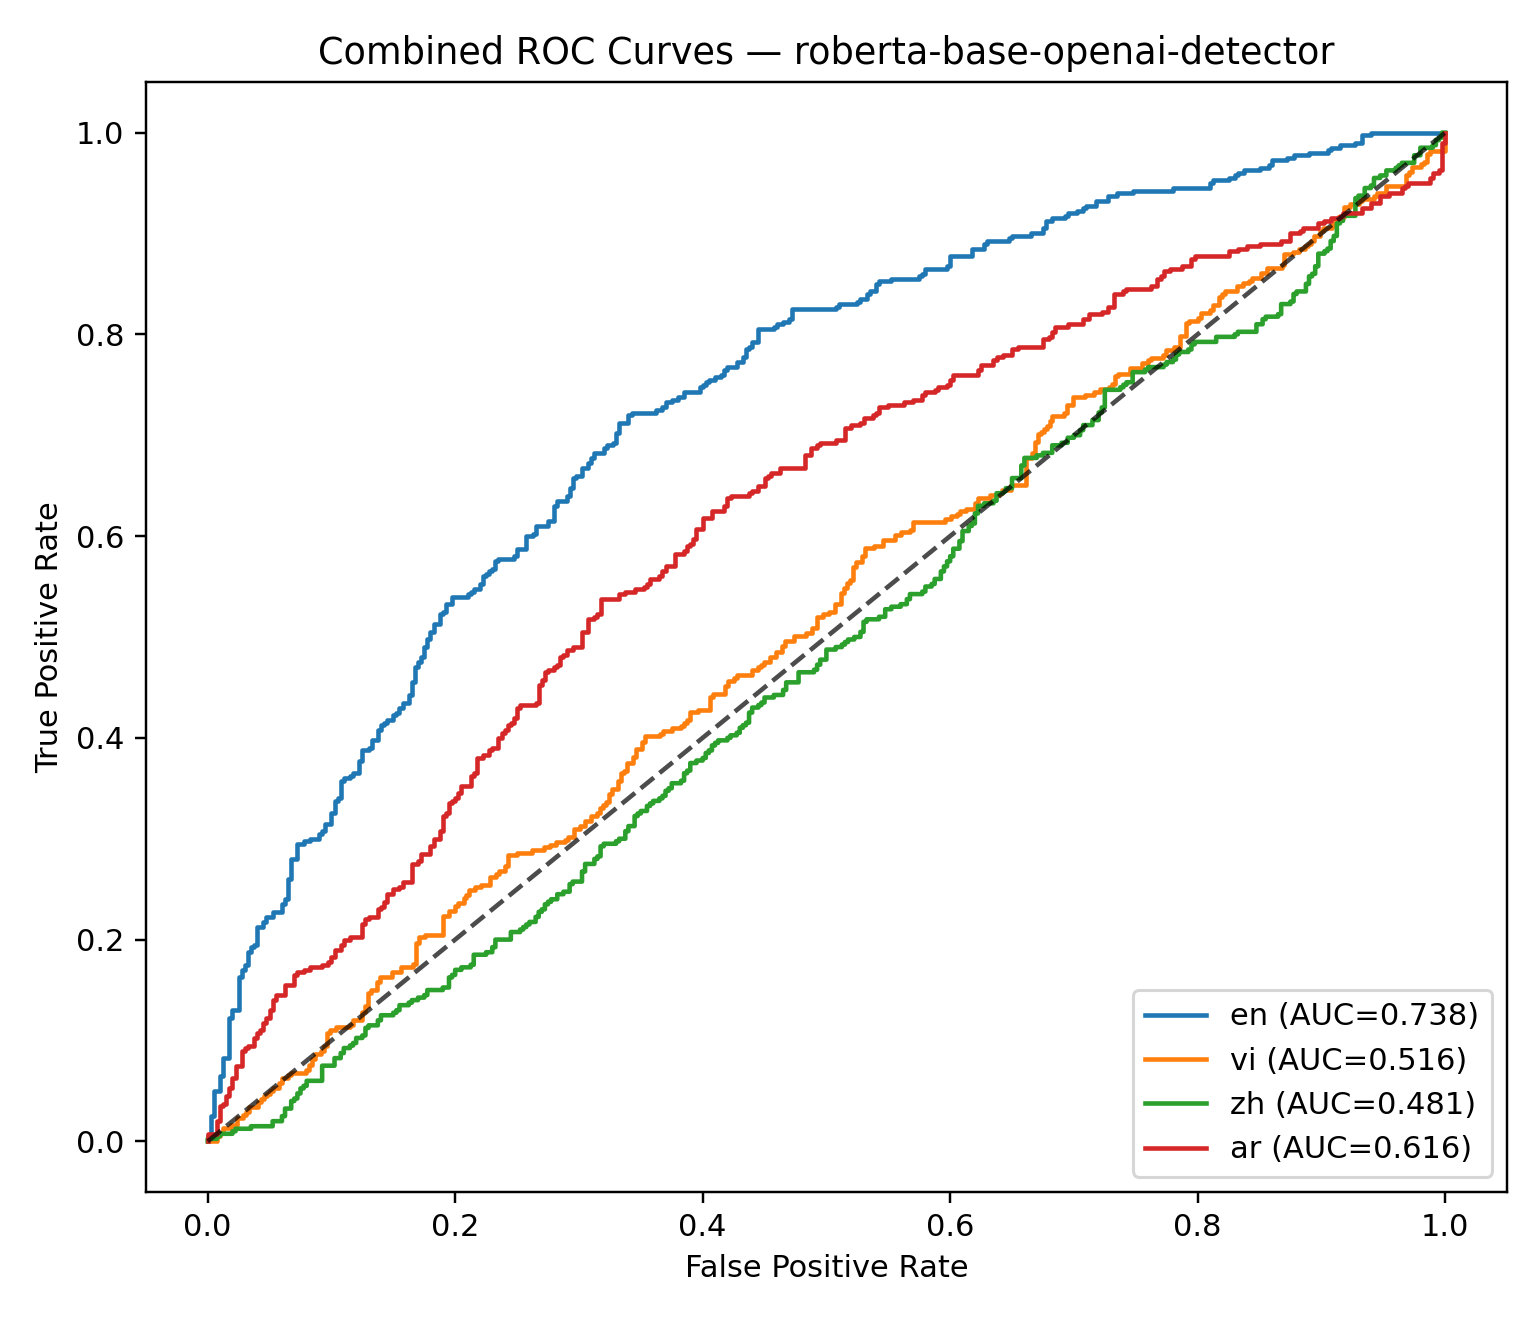
\includegraphics[width=0.75\textwidth]{roc_baseline.png}
\caption{Đường cong ROC --- Baseline (roberta-base-openai-detector).
Chỉ EN đạt AUC khả dụng (>0.6); AR, VI, ZH gần như ngẫu nhiên.}
\label{fig:roc_baseline}
\end{figure}

\subsection{Kết Quả Tinh Chỉnh XLM-RoBERTa}

Sau khi tinh chỉnh trên 12.789 mẫu đa ngôn ngữ, hiệu năng cải thiện
đáng kể trên tất cả bốn ngôn ngữ (Bảng~\ref{tab:finetuned}). Mức tăng
trung bình ước tính là \textbf{+28,7 điểm phần trăm} so với baseline.

\begin{table}[h]
\centering
\caption{Kết quả Phương pháp 2: Tinh Chỉnh XLM-RoBERTa (xlm-roberta-base)}
\label{tab:finetuned}
\begin{tabular}{lrrrr}
\toprule
\textbf{Ngôn ngữ} & \textbf{Accuracy} & \textbf{Macro-F1} & \textbf{N test}
    & \textbf{$\Delta$ Acc} \\
\midrule
EN & \textbf{95,4\%} & 0,954 & 800  & +31,3 pp \\
VI & 70,3\%          & 0,702 & 797  & +19,6 pp \\
ZH & 71,5\%          & 0,712 & 800  & +23,9 pp \\
AR & \textbf{88,3\%} & 0,882 & 800  & +40,0 pp \\
\midrule
\textbf{Tổng} & \textbf{81,4\%} & \textbf{0,814} & 3.197 & \textbf{+28,7 pp} \\
\bottomrule
\end{tabular}
\end{table}

Tiếng Ả Rập đạt mức tăng lớn nhất (+40,0 pp), từ trạng thái ``phân
loại sai hệ thống'' lên 88,3\% --- cho thấy XLM-RoBERTa đã học được
các đặc trưng hình thái của tiếng Ả Rập một cách hiệu quả. Tiếng Việt
và tiếng Trung đạt khoảng 70--72\%, thấp hơn đáng kể so với EN và AR,
phản ánh độ khó nội tại: Teencode trong tiếng Việt và văn bản Weibo cực
ngắn (15--30 ký tự) trong tiếng Trung. Hình~\ref{fig:roc_finetuned} hiển
thị đường cong ROC sau tinh chỉnh.

\begin{figure}[h]
\centering
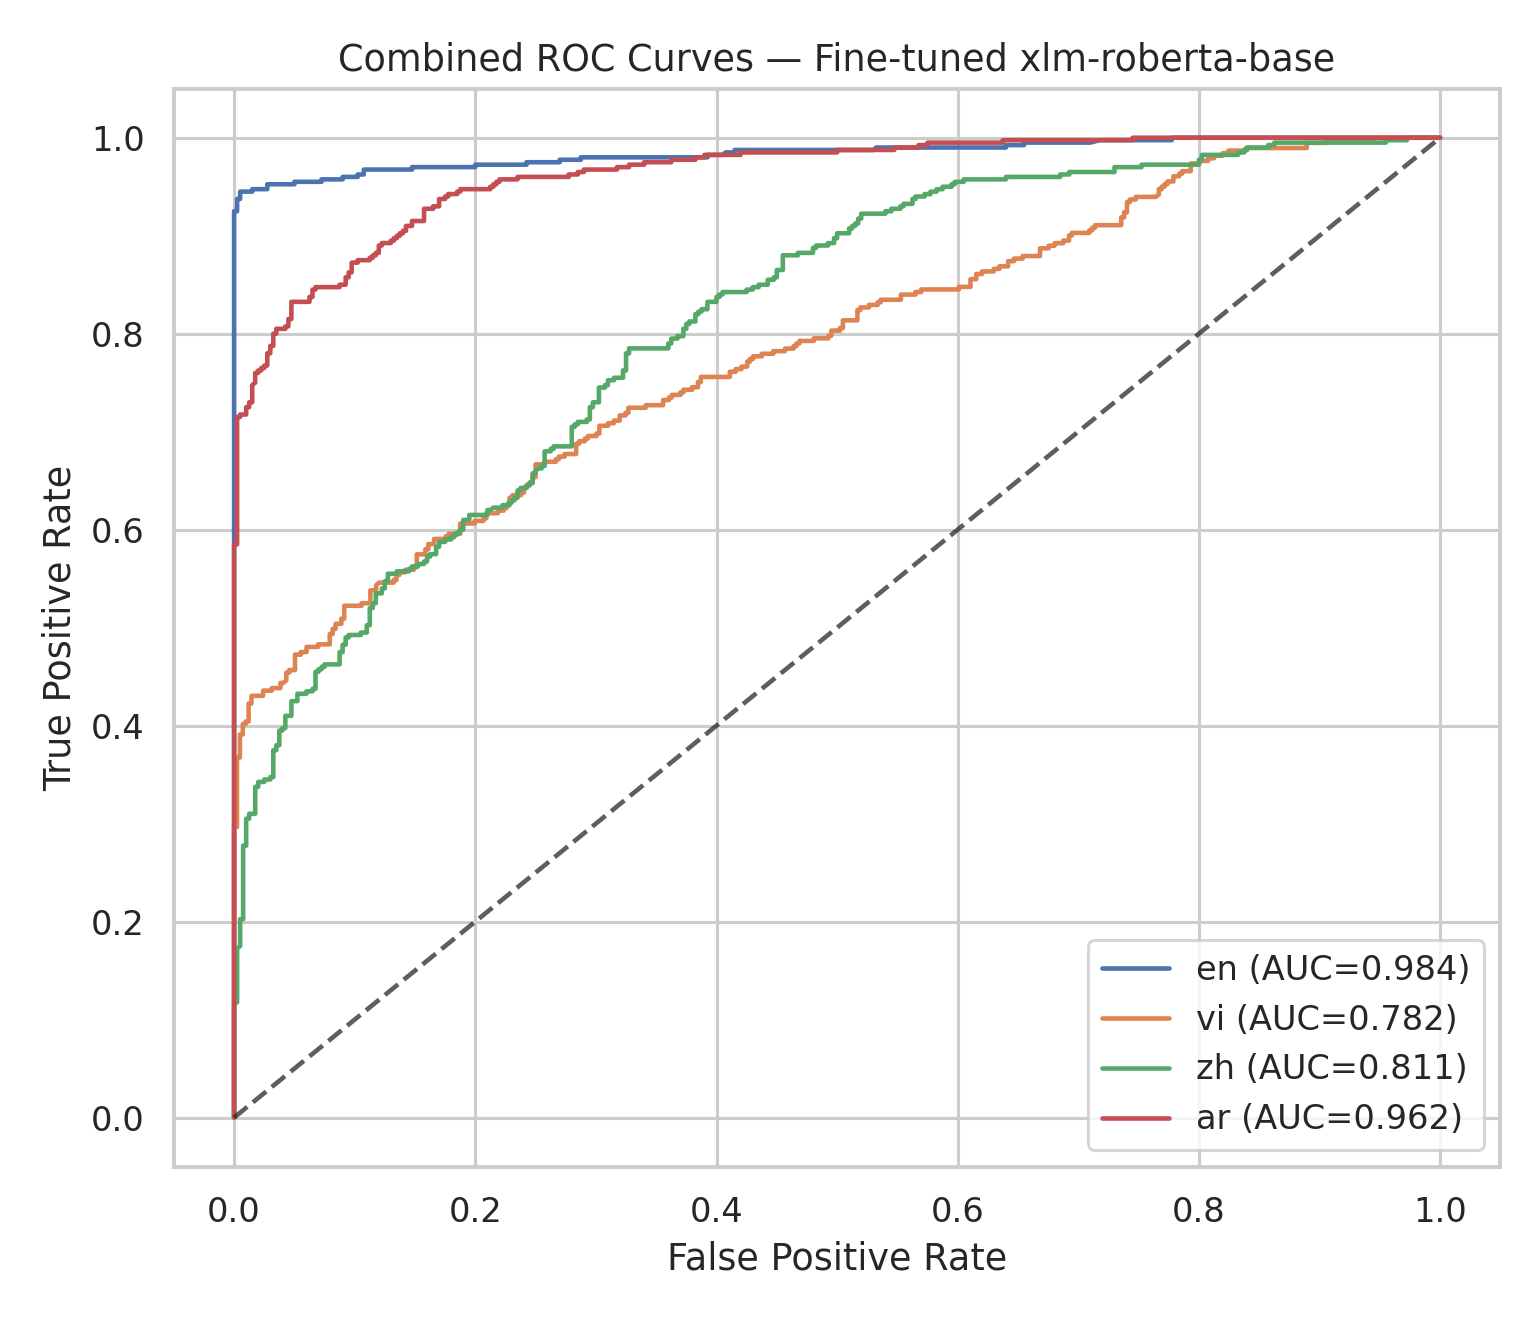
\includegraphics[width=0.75\textwidth]{roc_finetuned.png}
\caption{Đường cong ROC --- XLM-RoBERTa sau tinh chỉnh.
EN và AR đạt AUC gần hoàn hảo (>0.95); VI và ZH cải thiện đáng kể so với baseline.}
\label{fig:roc_finetuned}
\end{figure}

\subsection{Kết Quả Phát Hiện Dựa Trên Perplexity}

Bảng~\ref{tab:ppl} và Hình~\ref{fig:roc} trình bày kết quả phương pháp
PPL. EN (AUC = 0,754) và AR (AUC = 0,778) đạt hiệu năng khá tốt, trong
khi VI (AUC = 0,538) và ZH (AUC = 0,534) gần như ngẫu nhiên.

\begin{table}[h]
\centering
\caption{Kết quả Phương pháp 3: Perplexity Zero-Shot (Qwen2.5-1.5B)}
\label{tab:ppl}
\begin{tabular}{lrrrrl}
\toprule
\textbf{Ngôn ngữ} & \textbf{AUC-ROC} & \textbf{PPL\textsubscript{Human}}
    & \textbf{PPL\textsubscript{Machine}} & \textbf{Tỉ lệ} & \textbf{Đánh giá} \\
\midrule
EN & \textbf{0,754} & 1.193,6 & 187,1  & 6,4$\times$ & Tốt \\
AR & \textbf{0,778} & 260,7   & 76,7   & 3,4$\times$ & Tốt \\
VI & 0,538          & 1.210,4 & 796,0  & 1,5$\times$ & Yếu \\
ZH & 0,534          & 221,5   & 207,9  & 1,07$\times$ & Ngẫu nhiên \\
\bottomrule
\end{tabular}
\end{table}

\begin{figure}[h]
\centering
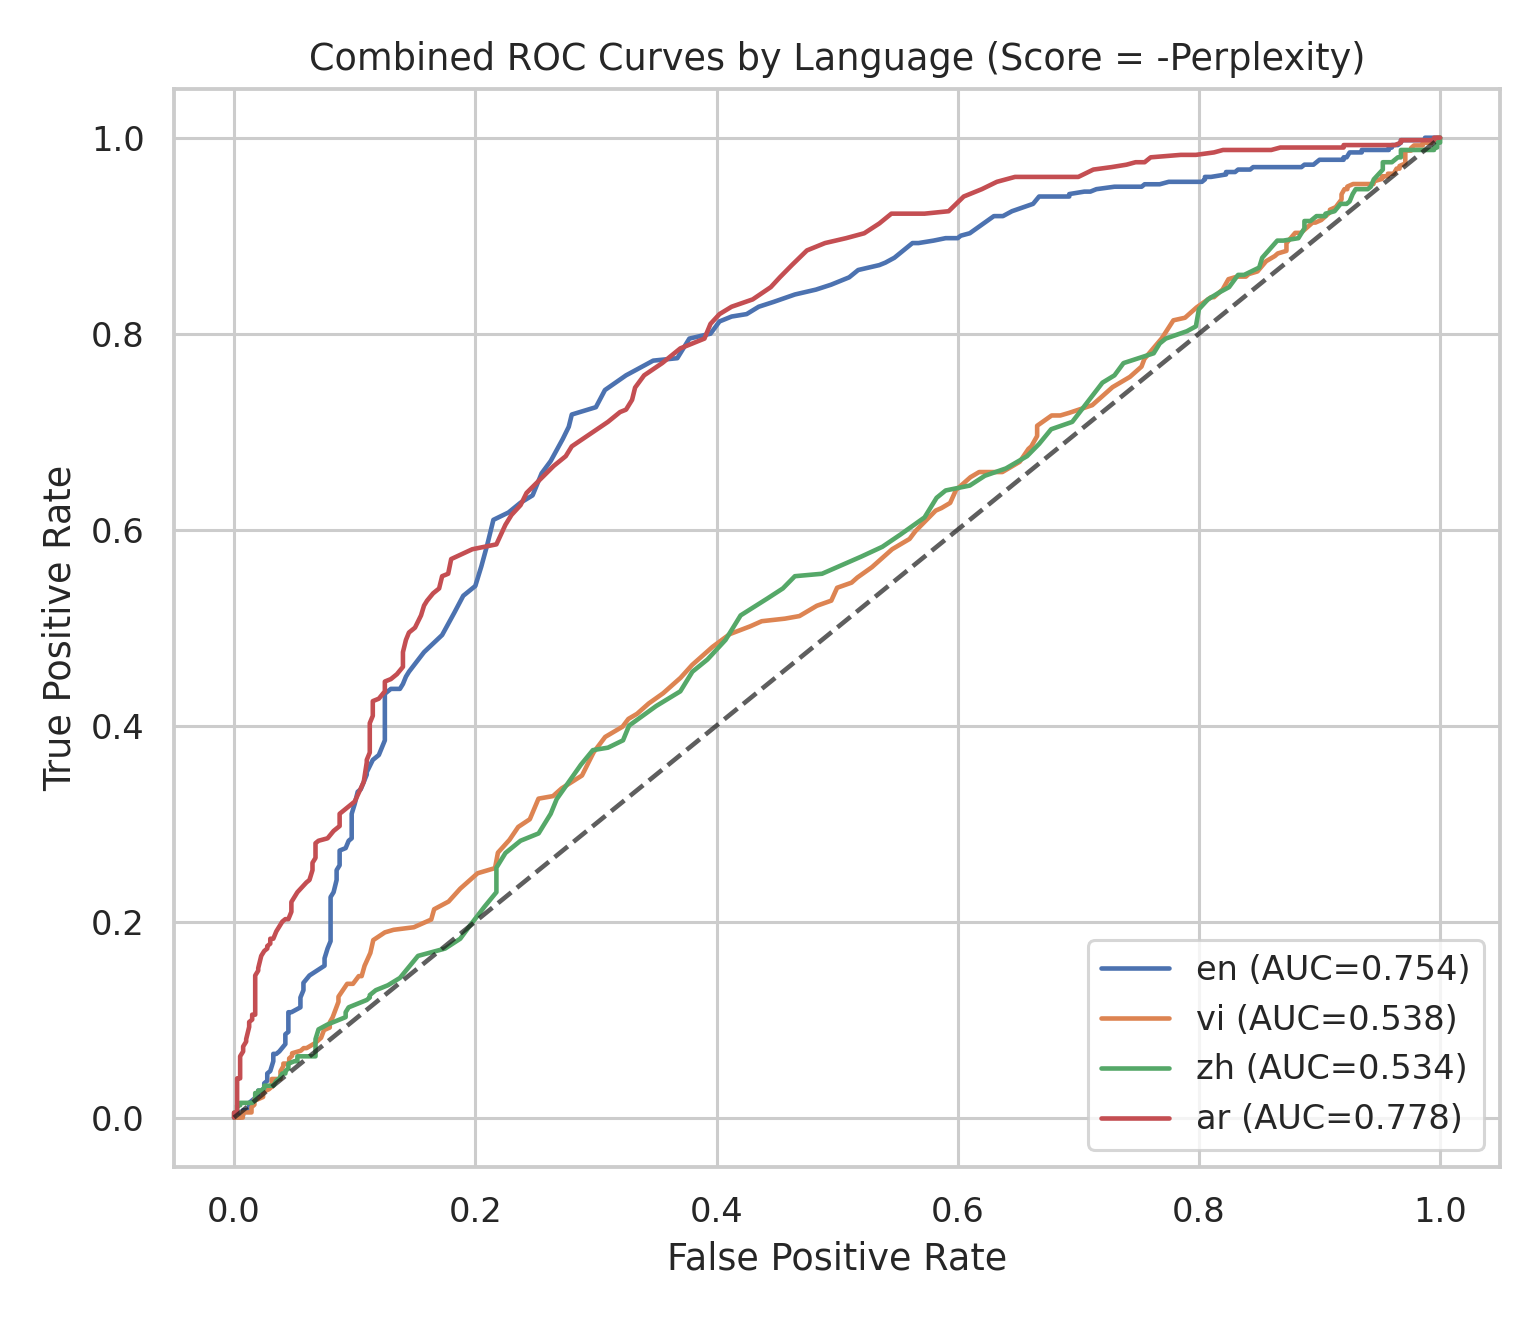
\includegraphics[width=0.75\textwidth]{roc_statistical.png}
\caption{Đường cong ROC của phương pháp PPL (Qwen2.5-1.5B) trên 4 ngôn ngữ.
EN và AR có đường cong gần góc trên trái; ZH gần như trùng đường chéo ngẫu nhiên.}
\label{fig:roc}
\end{figure}

Hiệu năng kém của VI và ZH được lý giải qua tỉ lệ PPL: ZH chỉ đạt
\textbf{1,07$\times$} --- con người và máy hầu như không phân biệt được
qua PPL --- do bài đăng Weibo cực ngắn khiến cả hai lớp có entropy tương
đương nhau. VI đạt 1,5$\times$ nhưng chưa đủ lớn để phân tách tốt, do
Teencode làm tăng PPL đồng đều cho cả hai lớp.

\subsection{Kết Quả Học Chuyển Giao (Transfer Learning)}

Bảng~\ref{tab:transfer} trình bày kết quả của bốn thí nghiệm
\textit{leave-one-language-out}. Hiệu năng trung bình chỉ đạt
\textbf{54,9\% accuracy} và \textbf{0,543 F1}, gần với mức ngẫu nhiên.

\begin{table}[h]
\centering
\caption{Kết quả học chuyển giao (xlm-roberta-base, leave-one-language-out)}
\label{tab:transfer}
\begin{tabular}{lcccc}
\toprule
\textbf{Ngôn ngữ} & \textbf{Ngôn ngữ huấn luyện} & \textbf{Acc}
    & \textbf{F1} & \textbf{ROC-AUC} \\
\midrule
EN & VI, ZH, AR & 0,545 & 0,683 & 0,851 \\
VI & EN, ZH, AR & 0,531 & \textbf{0,134} & 0,536 \\
ZH & EN, VI, AR & 0,503 & 0,666 & 0,512 \\
AR & EN, VI, ZH & \textbf{0,619} & 0,691 & \textbf{0,810} \\
\midrule
\textbf{Trung bình} & & \textbf{0,549} & \textbf{0,543} & \textbf{0,677} \\
\bottomrule
\end{tabular}
\end{table}

Kết quả cho thấy ba hiện tượng đáng chú ý:

\begin{enumerate}
    \item \textbf{Tiếng Việt thất bại hoàn toàn} (F1 = 0,134, recall = 0,076):
    Mô hình dự đoán gần như toàn bộ là ``human'', cho thấy đặc trưng
    MGT tiếng Việt (Teencode, cấu trúc câu không chính thức) không thể
    học được từ các ngôn ngữ khác.

    \item \textbf{Tiếng Trung bị thoái hóa} (Acc = 50,3\%): Mô hình thiên
    về nhãn ``machine'' (395/400 human bị phân loại sai), dẫn đến recall
    cao giả tạo (0,99) nhưng precision ngang tung đồng (0,501).

    \item \textbf{EN và AR được hưởng lợi một phần}: AR đạt kết quả tốt
    nhất (Acc = 61,9\%, AUC = 0,81). EN đạt recall 0,98 nhưng precision
    chỉ 0,524 --- thiên lệch về nhãn ``machine''.
\end{enumerate}

\subsection{So Sánh Tổng Hợp Bốn Phương Pháp}

Bảng~\ref{tab:comparison} tổng hợp hiệu năng của bốn phương pháp.

\begin{table}[h]
\centering
\caption{So sánh tổng hợp bốn phương pháp}
\label{tab:comparison}
\begin{tabular}{lrrrr}
\toprule
\textbf{Ngôn ngữ} & \textbf{Baseline Acc} & \textbf{XLM-R Acc}
    & \textbf{PPL AUC} & \textbf{Transfer Acc} \\
\midrule
EN & 64,1\% & \textbf{95,4\%} & 0,754 & 54,5\% \\
VI & 50,7\% & \textbf{70,3\%} & 0,538 & 53,1\% \\
ZH & 47,6\% & \textbf{71,5\%} & 0,534 & 50,3\% \\
AR & 48,3\% & \textbf{88,3\%} & 0,778 & 61,9\% \\
\midrule
\textbf{Khả dụng} & Chỉ EN & \textbf{4 ngôn ngữ} & EN + AR & Không \\
\bottomrule
\end{tabular}
\end{table}

XLM-RoBERTa tinh chỉnh là phương pháp vượt trội nhất trên tất cả ngôn
ngữ và tiêu chí. Phương pháp PPL có ưu điểm zero-shot (không cần dữ
liệu nhãn) và hiệu quả với EN/AR, nhưng thất bại với VI/ZH. Baseline
tiếng Anh không thể dùng được cho bài toán đa ngôn ngữ. Học chuyển giao
cho thấy mỗi ngôn ngữ cần dữ liệu huấn luyện riêng --- đặc biệt với
các ngôn ngữ có đặc thù hình thái như tiếng Việt và tiếng Trung.


% ---------- Section 6: Conclusion ----------
% ============================================================
%  sections/06_conclusion.tex
%  6. Kết luận & Hướng phát triển  (~0.5 trang)
% ============================================================

\section{Kết Luận và Hướng Phát Triển}
\label{sec:conclusion}

Bài báo này trình bày nghiên cứu so sánh hệ thống bốn phương pháp phát
hiện văn bản do máy tạo ra (MGT) trên dữ liệu mạng xã hội đa ngôn ngữ
gồm bốn ngôn ngữ: EN, VI, ZH, AR. Bốn kết luận chính được rút ra:

\begin{enumerate}
    \item \textbf{Thiên lệch Anh ngữ là nghiêm trọng và nguy hiểm:}
    Bộ phát hiện tiền huấn luyện chỉ dành cho tiếng Anh (\texttt{roberta-base-openai-detector})
    đạt dưới mức ngẫu nhiên trên VI, ZH, AR --- thậm chí phân loại sai
    hệ thống với AR (F1 = 0,336). Triển khai detector đơn ngôn ngữ cho
    bài toán đa ngôn ngữ là không thể chấp nhận được.

    \item \textbf{Tinh chỉnh XLM-RoBERTa là giải pháp thực tế tối ưu:}
    Đạt \textbf{81,4\% accuracy} trung bình, huấn luyện trong 7,5
    phút trên GPU T4 thông thường với chi phí ước tính \textbf{\$1,50}.
    Phương pháp này chứng minh rằng phát hiện MGT đa ngôn ngữ chất lượng
    cao không đòi hỏi phần cứng A100 đắt tiền.

    \item \textbf{PPL zero-shot hữu ích có điều kiện:}
    Phát hiện dựa trên perplexity (Qwen2.5-1.5B) hoạt động tốt khi tỉ
    lệ PPL giữa hai lớp đủ lớn (EN: 6,4$\times$, AR: 3,4$\times$), nhưng
    thất bại với văn bản MXH nhiễu (VI Teencode, ZH Weibo ngắn).

    \item \textbf{Học chuyển giao liên ngôn ngữ là chưa đủ:}
    Thí nghiệm leave-one-language-out cho thấy mỗi ngôn ngữ cần dữ liệu
    huấn luyện riêng. Tiếng Việt đặc biệt khó khăn (F1 = 0,134 khi
    không có dữ liệu VI trong tập huấn luyện), khẳng định tính tất yếu
    của dữ liệu đa ngôn ngữ trong bài toán MGT trên MXH.
\end{enumerate}

\subsection*{Hướng Phát Triển}

Nghiên cứu tiếp theo có thể khai thác các hướng sau:

\begin{itemize}
    \item \textbf{Mô hình cấp ký tự} cho VI và ZH nhằm xử lý đặc tính
          Teencode và bài đăng siêu ngắn (15--30 ký tự).
    \item \textbf{Data augmentation} với Teencode giả lập để cải thiện
          khả năng tổng quát hóa trên VI.
    \item \textbf{Mô hình lớn hơn với quantization:} thử nghiệm XLM-R
          large (559M) hoặc mGPT với INT8/INT4 quantization trên T4.
    \item \textbf{Mở rộng ngôn ngữ:} Thêm tiếng Nhật, Hàn, Hindi ---
          các ngôn ngữ MXH lớn chưa được nghiên cứu kỹ trong bài toán MGT.
    \item \textbf{Phát hiện cấp đặc trưng ngôn ngữ học:} kết hợp PPL
          với đặc trưng cú pháp và ngữ nghĩa để vượt qua giới hạn của
          phương pháp thuần PPL.
\end{itemize}

Mã nguồn, bộ dữ liệu và pipeline thực nghiệm sẽ được công khai để
thúc đẩy nghiên cứu tái lập và mở rộng.


% ---------- References ----------
\bibliographystyle{splncs04}
\bibliography{sections/references}

\end{document}
